The area/study of dilute Bose gases has been a field of research with great many discoveries over the last decades. The fact that microscopic quantum phenomena can be observed at a macroscopic level, compared to an atomic one, makes it an interesting subject in it self. With the improvement of laser cooling techniques there has been an explosion of discoveries and verification of theories of dilute Bose gases. Some of which include cold atomic gases of Rubidium-87, Sodium-23 and Lithium, (reference) 1995.

In dilute gases the scattering length is shorter than the inter-particle spacing. If we compare the molecule density in air at room temperature and atmospheric pressure which is $10^{19}$ cm$^{-3}$ to the density of a dilute gas at about $10^{14}$ cm$^{-3}$, the difference is enormous.

However, in order to observe quantum effects at such low densities, we must require low temperatures. Helium liquid must be cooled to the order of 1 K, absolute zero in order for effects to occur. This compared to electrons in metals which show quantum effects below the Fermi temperature, $10^4 - 10^5$ K. 
For the atomic nuclei the density is so high that degeneracy happens at temperature close up to $10^{11}$ K.

Bose-Einstein condensation in dilute gases occurs when the temperature is so low that $\lambda_T$, the thermal de Broglie wavelength, is comparable to the mean interparticle spacing, $n^{-1/3}$ \cite{BECCondInDilute}.

\begin{equation}
\lambda_T = \left( \frac{2 \pi \hbar^2}{m k T} \right)^{1/2}
\end{equation}

If $T$ is high then $\lambda_T$ is small, and the gas behaves classically. 

Working with dilute gases gives us the opportunity to approximate the system by a mean-field approach using Hartree-Fock theory. This is the basis of the Gross-Pitaevskii equation, the foundation of the studies of the Bose-Einstein condensate. It is an equivalence to the Schrödinger equation.

Maybe specify some constants if that is necessary. 

Application in condensed-matter physics, fluid mechanics, atomic and nuclear physics.

\section{Bose-Einstein Condensate}

The Bose-Einstein condensate (BEC) is the state of a dilute Bose gas at low temperatures at which most of the particles in the gas all resides the same quantum state. This was predicted by Albert Einstein in 1925 after taking the work of Satyendra Nath Bose, studying the statistics of photons, further. He considered a non-interacting gas of bosons at low temperature and concluded that the particles could all be found in the lowest-energy single-particle state. Together with Bose he formed the foundation of Bose-Einstein statistics which describes the statistical distribution of bosons. Before looking closer at the statistics in thermodynamics it can be practical to explain what a boson is.

\subsection{Bosons and fermions}
Bosons are particles with integer spin. They can be fundamental particles like the photon or gluon. But also composite particles like mesons or the stable isotope of the helium atom, $^4\text{He}$. They posses the ability to occupy the same quantum state, unlike fermions which are particle of half-integer spin. Fermions include all quarks and leptons, but as bosons they can also be composite particles, like $^3\text{He}$. They underlay the Pauli exclusion principle. It states that two or more identical fermions can not occupy the same quantum state. 
The typical example being two electrons occupying the same orbital in an atom must have opposite spin quantum number as they have same quantum numbers otherwise. 
This principle leads to fermions being governed by the Fermi-Dirac statistics and bosons by the Bose-Einstein statistics. 

% Add some single particle basis vectors
% explain the symmetric and antisymmetric solutions?

We will come back to this, but first, lets look at one of the most important formulas in statistical mechanics. 

\subsection{Particle statistics}

OBS: lese om partition function i boka hjemme!


Picture a system in thermal equilibrium with a reservoir with temperature T, a canonical system. Then we know from thermal physics that the probability of finding a system in any particular microstate $s$ with energy $E(s)$ is given by \eqref{eq:prob_boltzmann}.

\begin{equation} \label{eq:prob_boltzmann}
P(s) =  \frac{1}{Z} e^{-E(s)/kT}    
\end{equation}

The exponent is the Boltzmann factor, $e^{-E(s)/kT}$, where $k$ is the Boltzmann constant and $T$ the temperature of the reservoir. $Z$ is called the \textit{partition function}, the sum over all Boltzmann factors i.e. the sum over all states. This is easily seen if we use the fact that the sum of all possibilities must equal 1. The particle must be in one of the states. 

%Average values: page 230 thermal physics

\begin{equation}
1 = \sum_s P(s) = \sum_s \frac{1}{Z} e^{-E(s)/kT} = \frac{1}{Z} \sum_s e^{-E(s)/kT}
\end{equation}

If we now look at a system where the system is allowed to exchange particles with the environment as well as the energy, the factor in the exponential changes. And we end up with the Gibbs factor. 

\begin{equation}
\text{Gibbs factor} = e^{-[E(s) - \mu N(s)]/kT}
\end{equation}

We are now looking at a grand canonical system, and the partition function from before is now a grand partition function.
Now we can calculate the probability of a system containing N particles being in the state s(N) with corresponding energy E(s).
$\mu$ being the chemical potential of the reservoir that is effectively constant, T also constant.

\begin{equation}
P(n) = \frac{1}{Z} e^{-n(\epsilon - \mu)/kT}
\end{equation}

We want to find the average number of particles being in one energy state $\epsilon_{\mu}$, i.e. the distribution of particles over energy states. Lets consider the probability of a particle occupying a single-particle state. 

If we begin looking at fermions, we know they obey the Pauli exclusion principle, and the grand partition function for the one particles is given by \eqref{eq:partition_fermion}.

\begin{equation} \label{eq:partition_fermion}
Z = 1 + e^{-(\epsilon - \nu)/kT}
\end{equation}

Since the particle can either occupy the state or not we get the following.

\begin{equation}
\overline{n} = \sum_n n P(n) = \frac{e^{-(\epsilon - \mu)/kT}}{ 1 + e^{-(\epsilon - \mu)/kT}} = \frac{1}{e^{-(\epsilon - \mu)/kT} + 1}
\end{equation}

Forklar denne funksjonen...

\begin{equation}
\overline{n}_{FD} = \frac{1}{e^{(\epsilon_{\nu} - \mu)/kT} + 1}
\end{equation}

Since bosons can occupy the same state, the partition function  for bosons becomes different. 

\begin{equation}
Z = \frac{1}{1 - e^{-(\epsilon - \mu)/kT}}
\end{equation}

Also now we 

\begin{equation}
\overline{n} = \sum_n n \frac{e^{-nx}}{Z} = -\frac{1}{Z} \sum_n \frac{\partial}{\partial x} e^{-nx} = -\frac{1}{Z} \frac{\partial Z}{\partial x}
\end{equation}

Here $x \equiv (\epsilon_{\nu} - \mu)/kT$

\begin{equation}
\overline{n}_{BE} = \frac{1}{e^{(\epsilon_{\nu} - \mu)/kT} - 1}
\end{equation}

Now we have come to quantum statistics.
The average number of particles being in an energy state $\epsilon_{\nu}$.

For non-interacting particles in thermodynamic equilibrium the mean occupancy number is given by the Boltzmann distribution.

\begin{equation}
\overline{n}_{Boltzmann} = e^{-(\epsilon_{\nu} - \mu)/kT}
\end{equation}

\begin{figure}
    \centering
    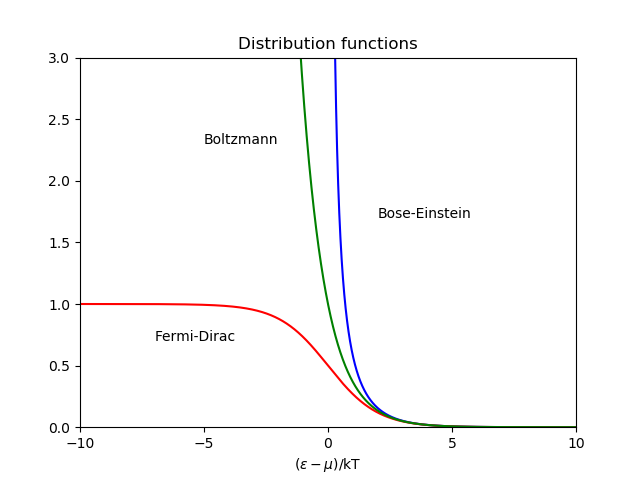
\includegraphics[width=0.7\textwidth]{images/distributions.png}
    \caption{Fermi-Dirac dist. goes to 1 for $\epsilon_{\nu} \gg \mu$}
    \label{fig:dist_therm_stat}
\end{figure} 
s269

In the case of Bose-Einstein: as temperature decreases, $\epsilon - \mu$ goes to zero ($\epsilon$ goes to $\mu$), the distribution diverges. The particles occupy the ground state.

Fermi-Dirac: as T increases towards 0, the distribution becomes a step-function.

Read further page 251 Thermal Physics \cite{ThermalPhysics}
When $\epsilon_{\nu}$ is much greater than $\mu$ the term $\pm 1$ in the denominator of both expressions and they reduce to the Boltzmann distribution. 


\subsection{The ideal Bose gas}

Uniform density: particles in a box with voloum V.
Density inside box: n = N/V

Classical case, use Boltzmann distribution
The termodynamics of an ideal Bose gas is best calculated using the grand canonical ensamble. Then the partition function is 

\begin{equation}
Z(\mu, \beta, V) = \prod_i (1 - \mu e^{(-\beta \epsilon_i)})^{g_i}
\end{equation}

Is This correct?? Check book

Ground state energy

The ideal bose gas is straight forward and have been solved analytically and numerically by many. Weak interacting bosons is also a case that has been studied to a great extent. If we where to add strong interaction the system may do a number of things, flipping of spin, excitation etc.


The ability of bosons at low temperature to collectively inhabit the same energy state, compared to fermions who are restricted to the Pauli exclusion principle.

Free Bose gas - 

\begin{equation} \label{eq:hamilt_free_bose_gas}
H^{free}_V = \int_V dx \frac{1}{2m} \nabla a*(x). \nabla a(x)
\end{equation}


\section{Bose gas in a trap}

As mentioned above, methods for trapping and cooling alkali atom clouds have developed over the last decades, and these systems have been explored considerably. We will now look closet at a Bose gas confined within such a trap and look at the properties of the condensate.
For the BEC the theoretical framework lies within the Gross-Pitaevskii equation, derived by Eugene P. Gross and Lev Petrovich Pitaevskii each in therir own separately papers, 1961.


The Gross-Pitaevskii equation form the basis of studies of dilute Bose gases at zero temperature. It gives the ground-state energy of a system of identical bosons.

Trap: a harmonic oscillator potential trap. 

Consider a dilute Bose gas where the inter-particle distance is much greater than the scattering length. It can be approximated by a mean field theory. We describe it by a simple hard-sphere effective potential. (Master Joachim)

Gross-Pitaevskii - analogy to the Schrödinger equation. 

\subsection{The Gross-Pitaevskii equation}

The time-independent Gross-Pitaevskii equation reads as follows

\begin{equation} \label{Gross-Pitaevskii}
\left( -\frac{\hbar^2}{2m} \frac{\partial^2}{\partial r^2} + V(r) + \frac{4 \pi \hbar^2 a_s}{m}|\psi(r)|^2 \right) \psi(r) = \mu \psi (r)
\end{equation}

For a uniform Bose gas, the GP equation is very simple.

\begin{equation}
\mu = U_0 |\psi (\textbf{r})|^2 = U_0n
\end{equation}

Where $\mu$ being the chemical potential.

page 114
cut-off $k_c$

page 146 equations!

The Bose-Einstein condensation ground state can be described by the Gross-Pitaevskii equation, which uses the Hartree-Fock approximation and the pseduopotential intereaction model. (wiki) 
A a many-body boson system, the Gross-Pitaevskii approach is a mean-field approach. (MBBS)
If the spacing between the particles are greater than the scattering length (in the so-called dilute limit), then one can approximate the true interaction potential that features in this equation by a psedopotential.

READ more about why this is.

Psedopotential: a contact interaction $U_0 \delta(r_i - r_j)$
with $U_0 = \frac{4 \pi \hbar^2 a}{m}$.
We can assume this if the energy is low, zero-temperature, when scattering lenght is much less than the mean interparticle spacing. 
This makes it a mean-field potential. 

The total wave function in the Hartree-Fock approximation of a system of N bosons is represented by the product of single-particle wave functions $\phi$

\begin{equation}
\psi(r_1, r_2, \cdots, r_N) = \phi(r_1) \phi(r_2) \cdots \phi(r_N)
\end{equation}

The pseudopotential model Hamiltonian of the system is given as 

\begin{equation}
H = \sum_{i=1}^N \left( -\frac{\hbar^2}{2m} \frac{\partial^2}{\partial r_i^2} + V(r_i) \right) + \sum_{i<j} \frac{4 \pi \hbar^2 a_s}{m} \delta (r_i - r_j)
\end{equation}

m is the mass of the boson, V is the external potential, $a_s$ is the boson-boson scattering length and $\delta(r)$ the Dirac delta-function. This is an effective potential, the original  with modifications 

The Gross-Pitaevskii equation reads, 

\begin{equation}
\left( -\frac{\hbar^2}{2m} \frac{\partial^2}{\partial r^2} + V(r) + \frac{4 \pi \hbar^2 a_s}{m}|\psi(r)|^2 \right) \psi(r) = \mu \psi (r)
\end{equation}

Se 104 MBBS

Solutions: free particle V(r) = 0

Soliton?

Thomas-Fermi approximation

Bogoliubov approximation: transformation to diagonalize Hamiltionian, yields the stationary solution of the Schrödinger equation. When one must go beyond mean-field theory. 

Interacting Bose gas - Landau's phenomenological theory of superfluidity. Based on the idea that a quantum liquid remains a classical fluid even at zero temperature  and that the classical hydrodynamical laws remain valid. (Many body boson system.) 
Many models have been suggested to create a microscopical theory of the superfluidity. Vortex ring model, hard-sphere model, guassian cluster approach. (wiki)

The properties of these liquids are described in terms of the spectrum of the collective excitations.

\subsection{The wave function}
We are studying a system of two electrons confined in a harmonic oscillator trap described by the Hamiltonian 

\begin{equation}\label{eq:hamilt_trap}
\hat{H} = \sum_{i=1}^N \left( - \frac{1}{2} \nabla_i^2 + \frac{1}{2} \omega^2 r_i^2 \right) + \sum_{i<j} \frac{1}{r_{ij}}
\end{equation}

where the first sum is the standard harmonic oscillator part and the last is the interacting part between the electrons and $N$ represent the number of particles. $\omega$ is the oscillator frequency of the trap and $r_i$ is the position of particle $i$, whereas $r_{ij}$ is the distance between the particles and given as $r_{ij} = |\mathbf{r_i} - \mathbf{r_j}|$. \\

\begin{equation} \label{eq:trap_potential}
 V_{ext}(\mathbf{r}) = 
 \Bigg\{
 \begin{array}{ll}
	 \frac{1}{2}m\omega_{ho}^2r^2 & (S)\\
 \strut
	 \frac{1}{2}m[\omega_{ho}^2(x^2+y^2) + \omega_z^2z^2] & (E)
 \end{array}
\end{equation}

\begin{equation} \label{eq:potential_internal}
 V_{int}(|\mathbf{r}_i-\mathbf{r}_j|) =  \Bigg\{
 \begin{array}{ll}
	 \infty & {|\mathbf{r}_i-\mathbf{r}_j|} \leq {a}\\
	 0 & {|\mathbf{r}_i-_r\mathbf{r}_j|} > {a}
 \end{array}
\end{equation}



\subsection{The ground-state energy}

\section{Strong interacting gases}

At low temperature, liquid helium ($^4$He) becomes a superfluid, but because of strong interactions it is difficult to treat microscopically. In stead one can turn to a hydrodynamical description. Toy model: BEC trests gases, but helium is the only known atom to remain liquid at low temp. 

Thermal physics book, page 168:
Phase shift of Helium-4: at low temp, below 2.2 K it turns to superfluid.
Above this temp. and pressure around 1 bar and up, it is normal liquid. For temp 

\subsection{Liquid $^4$He}
Due to the strong correlation between the atoms in liquid helium, a mean-field approach is inapplicable. Dilute gas, but still interaction plays an important role when temperature is so low. 
The interaction between Helium atoms is strong. Reduces the number of atoms in the zero-momentum state. 
Liquid helium does not solidify at low temperatures. At a threshold it becomes a superfluid, flow through narrow channels without friction. 

Landau: two-fluid description, one part the normal component and another part the superfluid component. 
At normal state the normal component is larger, and the superfluid comp. very small, for liquid helium only 10 percent or lower.
But the fractions are reversed at lower temp. lower then transition temp. 

Elementary excitations: quasiparticles or collective excitations

If quasiparticle is related to fermion, quasiparticle; electron holes (positively charged particles to represent an electron in a valence..)
Collectiv excitations if related to bosons: phonons (particle derived from vibration of atoms in solids) 
Liquid 4-Helium: the energy of dispersion $\epsilon = sp$ s being the velocity of sound and p the momentum.

\subsection{Lennard-Jones potential}


\begin{equation} \label{eq:hamilt_box}
\hat{H} = \sum_{i=1}^N - \frac{1}{2} \nabla_i^2  + \sum_{i<j} V(r)
\end{equation}

\begin{equation} \label{eq:lennard-jones}
V(r) = 4\epsilon \left[ \left( \frac{\sigma}{r} \right)^{12} - \left( \frac{\sigma}{r} \right)^6 \right]
\end{equation}
